\chapter{ Theoretical background }
\noindent At the end of the last chapter we announced that the problem we want to study in this document is that of ultra-orthogonality. Particularly, in the previous chapter, we showed how ultra-orthogonality is connected to the problem of equilibration as an instantaneous phenomenon. Since this problem is quite general, we focus our research to study the particular case in which ultra-orthogonality holds exactly for a particular kind of fermionic systems. For that reason, the purpose of this chapter is to provide the necessary theoretical background to study ultra-orthogonality for the aforementioned case.\\

\indent In this chapter we introduce the concepts of quasi-free fermionic models on a lattice and present Majorana fermions to define the fermionic covariance matrix. We show how this formalism can be used to develop some standard calculations on the diagonalisation of the Hamiltonian of the one-dimensional $XY$ model, and we will discuss how is possible to treat excited states as well as local reduced states in this model. Since part of this work is dedicated to show an explicit connection between a special case of fermionic systems and code theory, the second part of this chapter will be devoted to introduce some concepts of code theory that will allows us to make the explicit connection between code theory and fermionic system in the third chapter.

\section{Fermionic quadratic Hamiltonian}
In many areas of quantum physics one has to deal with solving problems systems of many body. However, the cases that can be analytically solved are well-known, and have been a subject of study of many authors\cite{noauthor_density_2007,niu_majorana_2012,reyes-lega_aspects_2016,chung_density-matrix_2001,leijnse_introduction_2012, molinari_notes_2017,botero_bcs-like_2004, bravyi_lagrangian_2004, lieb_two_1961, latorre_ground_2004, katsura_statistical_1962, barouch_statistical_1971, barouch_statistical_1970}.\\

\indent It has been found vast set of complicated Hamiltonians with many-body interactions can often be mapped onto Hamiltonians that are quadratic in annihilation and creation operators and have the generic form \cite{botero_bcs-like_2004}

\begin{equation}
\hat{H}=\sum_{i j} C_{i j} \hat{a}_{i}^{\dagger} \hat{a}_{j}+\sum_{i j}\left(A_{i j} \hat{a}_{i}^{\dagger}\hat{a}_{j}^{\dagger}+\mathrm{h.c.}\right),
\label{CH2:QuadraticHamiltonian}
\end{equation}

where $i,j$ run from $1$ to $N$, the number of modes in the system and $\hat{a}_i$, $\hat{a}^{\dagger}_i$ are fermionic annihilation and creation operators that satisfy the Fermi-Dirac commutation commutation relation also named simply as the canonical anti-commutation relations (CAR) \cite{fradkin_field_1997, Mario_2018}
\begin{equation}
\left\{\hat{a}_{k}, \hat{a}_{l}\right\}=\left\{\hat{a}_{k}^{\dagger}, \hat{a}_{l}^{\dagger}\right\}=0, \quad\left\{\hat{a}_{k}, \hat{a}_{l}^{\dagger}\right\}=\delta_{k l}.
\label{CH2:Anticommutation}
\end{equation}
These kind of Hamiltonians have the property that can be diagonalised via a Bogoliubov - Valantin transformation \cite{bogoljubov_new_1958,Mario_2018}, also known as a canonical transformation, which maps fermionic creation and annihilation operators to creation and annihilation operators of non-interacting quasi-particles \cite{berezin_method_1966, bogoljubov_new_1958}. Explicitly, the transformation looks like
\begin{equation}
\begin{array}{c}
\hat{a}_{i} \mapsto \alpha \hat{q}_{i}+\kappa_{i} \hat{q}_{i}^{\dagger}, \\
\hat{a}_{i}^{\dagger} \mapsto \bar{\alpha}_{i} \hat{q}_{i}^{\dagger}+\bar{\kappa}_{i} \hat{q}_{i}.
\end{array}
\label{CH2:Bogoliuvov}
\end{equation}
where $\alpha_i , \kappa_i$ are complex numbers such that preserves the canonical anti-commutation relations given by \eqref{ CH2:Anticommutation} for $\hat{q}$, $\hat{q}^{\dagger}$. This relation can also be expresses as a condition over $\gamma_i, \kappa_i$,
\begin{equation}
 \bar{\alpha}_i ^2+ \kappa_i^2 = 1,
\end{equation}
and 
\begin{equation}
	\left\{\hat{q}_{k}, \hat{q}_{l}\right\}=\left\{\hat{q}_{k}^{\dagger}, \hat{q}_{l}^{\dagger}\right\}=0, \quad\left\{\hat{q}_{k}, \hat{q}_{l}^{\dagger}\right\}=\delta_{k l}.
\end{equation}
The Bogoliubov-Valantin is relevant in many physics models because this transformation diagonalise many Hamiltonians; some examples of this are the Hubbard model, the BCS theory of superconductivity in the mean field or Hartree-Fock approximation, and certain solvable spin-chain models (After a Jordan-Wigner transformation) \cite{katsura_statistical_1962, barouch_statistical_1971, barouch_statistical_1970,fradkin_field_1997}.\\

\indent Hamiltonians with the form of \eqref{CH2:QuadraticHamiltonian} have the interesting property that not only the ground state but every eigenstate representing a certain number of excitations of quasi-particles, described by $\hat{a}$ and $\hat{a}^{\dagger}$, belong to the so-called class of fermionic Gaussian states, which is an interesting property, since it allows us to characterise them in terms of second order correlations, and the reason is because all the higher moments factorize as stated in Wick’s theorem \cite{westwanski_general_1973, molinari_notes_2017, Mario_2018,}. An equivalent but convenient characterization of second order correlations are defined in terms of Majorana fermions as we will see bellow \footnote{Taken from chapter $3$ of \cite{Mario_2018}}.

\section{Majorana Fermions}
Majorana fermions are represented in terms of $2N$ hermitian operators 
\begin{equation}
\hat{\gamma}_{j}=\hat{a}_{j}^{\dagger}+\hat{a}_{j+N}, \quad \hat{\gamma}_{j+N}=(-i)\left(\hat{a}_{j}^{\dagger}-\hat{a}_{j}\right),
\label{CH2:majorana}
\end{equation}
where these operators are analogous to coordinate and momentum operators for bosonic modes, and for each fermion labelled by $j$ of the original system we define two operators above. The canonical Fermi-Dirac commutation relation takes the form
\begin{equation}
\left\{\hat{\gamma}_{k},\hat{\gamma}_{l}\right\}=2 \delta_{k l}.
\label{CH2:CAR_majorana}
\end{equation}
The algebra generated by the operators $\{\hat{\gamma}_i\}$ is known as the Clifford algebra and is denoted by $\mathcal{C}_{2N}$\footnote{The orthogonal group in $2N$ dimensions $O(2N)$ preserves the Clifford algebra, hence, the canonical  canonical Fermi-Dirac commutation relations of fermionic operators}. When we change from the Fermionic operators $a^{T}:=(\hat{a}_,\hat{a}_2,\ldots,\hat{a}_N, \hat{a}^{\dagger}_1,\hat{a}^{\dagger}_2,\ldots,\hat{a}^{\dagger}_N)$ to Majorana operators $\gamma^{T}:=(\hat{\gamma}_1,\hat{\gamma}_2,\ldots, \hat{\gamma}_N,\hat{\gamma}_{N+1},\ldots,\hat{\gamma}_{2N})$, it is convenient to define the Fermionic covariance matrix which will fully characterise Gaussians states.  
%\footnote{In comparison to its boson counterpart the fermion Gaussian states have the property that correlation functions for the creation/annihilation operators are completely determined by the two-point functions according to Wick’s theorem \cite{westwanski_general_1973}, and moreover,  since this property is extensible to correlation function pertaining to a reduced subset of the modes, it follows that any partial (reduced) density matrix obtained from $\rho$ remains Gaussian.}.

\section{Fermionic Covariance matrix }
As we mentioned before, Gaussian states are completely characterised by its second moments \cite{westwanski_general_1973,molinari_notes_2017}, that is, Gaussian states have a density matrix $\rho$ \cite{cheong_many-body_2003},
\begin{equation}
\rho= \frac{1}{Z} \cdot \exp \left[-\frac{i}{4} \hat{\gamma}^{T} G \hat{\gamma}\right],
\label{CH2:rho_gaussiano_exp}
\end{equation}
with $\hat{\gamma} = (\hat{\gamma}_1,\hat{\gamma}_2,\ldots,\hat{\gamma}_{2N})$, the vector of Majorana operators \eqref{CH2:majorana}, $Z$ a normalization constant and $G$ real skew-symmetric $2N\times 2N$ matrix. Since $G$ is a skew-symmetric matrix, it can always be brought to the block diagonal form 
\begin{equation}
O G O^{T}=\left(\begin{array}{cc}
0 & -\tilde{B} \\
\tilde{B} & 0
\end{array}\right) \quad \text { with } \quad O \in \mathrm{SO}(2 \mathrm{N}),
\label{CH2:MatrixG_Williamson}
\end{equation}
where $\tilde{B}$ is diagonal, with eigenvalues that we denote by $\tilde{\beta}_k$. The right hand side of \eqref{CH2:MatrixG_Williamson} is known as the Williamson form of the skew-symmetric matrix $G$, and $\tilde{\beta}_k$ are the Williamson eigenvalues of $G$\cite{kraus_pairing_2009}.\\
\indent It is convenient to characterise second order correlations in terms of the so-called \textit{fermionic covariance matrix} (FMC), whose entries are
\begin{equation}
\Gamma_{k l}=\frac{i}{2} \operatorname{Tr}\left(\rho\left[\hat{\gamma}_{k}, \hat{\gamma}_{l}\right]\right),
\label{CH2:Cov_matrix_elements}
\end{equation}
where $\left[\hat{\gamma}_{k}, \hat{\gamma}_{l}\right] := \hat{\gamma}_{k}\hat{\gamma_{l}} - \hat{\gamma}_{l}\hat{\gamma}_{k}$. Thus, we can bring this anti-symmetric matrix to its block diagonal form, via a canonical transformation, as
\begin{equation}
\tilde{\Gamma} = O \Gamma O^{T}=\left(\begin{array}{cc}
0 & -\operatorname{diag}(\lambda_{i}) \\
\operatorname{diag}(\lambda_{i}) & 0
\end{array}\right),
\label{CH2:Williamson_Cov_fermionic_matrix}
\end{equation}
where $\lambda_k = \operatorname{tanh}(\tilde{\beta}_k/2)$, for $k=1,2\ldots,N$ \cite{kraus_pairing_2009}, which determines the connection between the matrix $G$ in \eqref{CH2:MatrixG_Williamson} and the FMC $\Gamma$. The Williamson eigenvalues are $\lambda_k=n_k -1/2$, with $n_k$ the fermion occupation number of the normal mode labelled by $k$. \\
\indent The equivalence between the special orthogonal group in $2N$ dimensions ($SO(2N)$) and the Fermionic Gaussian states, leads to an interesting  property about states describing multi-particles excitations. If $\ket{0}$ is the ground state of some Hamiltonian, with annihilation operators $\hat{a}_{i}$ in a given quasi-particle basis, then $\hat{a}_{i}^{\dagger}\ket{0} = \hat{c}_{2i}\ket{0}$. Meaning that if any multi-particle state of this kind is obtained from the ground state $\ket{0}$ through some transformation, such that preserves the canonical anti-commutation relation, the state will remain Gaussian. In other words, Gaussian states are preserved under any unitary transformation that preserves anti-commutation relations.\\
\indent The fact that all eigenstates of the Hamiltonian in \eqref{CH2:QuadraticHamiltonian} are Gaussian is an important property, because it means that excited states can also be treated with the Covariance matrix formalism, and since we will be interested in the case of the excited states, it will be a property that we will exploit.\\
\indent As an example of the afore-mentioned concepts, we will consider the case of the one-dimensional $XY$ model and we will see how is possible to characterise this system through the Fermionic covariance matrix. 
\section{$XY$ model.}
The $XY$ Hamiltonian model is a set of $N$ spin $1/2$ particles located on the sites of $d$-dimensional lattice. For the purpose of this document, whenever we refer to the $XY$ model, we will have in mind the $1D$ $XY$ model.\\
\indent A chain of $N$ spins where each spin is able to interact with its nearest neighbours in the $X$ and $Y$ component as well as an external magnetic field, will be described by the Hamiltonian of the form
\begin{equation}
H_{XY}=-\frac{1}{2} \sum_{l=0}^{N-1}\left(\frac{1+\gamma}{2} \hat{\sigma}_{l}^{x} \hat{\sigma}_{l+1}^{x}+\frac{1-\gamma}{2} \hat{\sigma}_{l}^{y} \hat{\sigma}_{l+1}^{y}+\lambda \hat{\sigma}_{l}^{z}\right),
\label{CH3:Hamiltonian_XY}
\end{equation}
where $\gamma$ is so-called the anisotropy parameter and represents the difference between the strength of the $XX$ interaction and the $YY$ interaction in the spin space, $\lambda$ is the intensity of the external magnetic field and
\begin{equation}
\hat{\sigma}^{i}_{l} = \mathbb{I}\otimes\cdots \otimes\mathbb{I}\otimes\underbrace{\hat{\sigma}^{i}}_{\text{site } l}\otimes\mathbb{I}\otimes\cdots\otimes\mathbb{I},
\end{equation}
where $\hat{\sigma}^{i}$ are Pauli matrices for $i=x, y, z$.
\subsection{The spectrum}
In order to find the spectrum of the of the $XY$ model, it is necessary to perform three different transformations. These results are very standard and we present them to make our discussion self-consistent.
\subsection{Jordan-Wigner transformation}
The Jordan-Wigner transformation is an important transformation used mainly in Fermionic systems  \cite{Michael_nielsen_2005}. The Jordan-Wigner transformation provides a bridge between spins and fermions through a non-local transformation that maps spin operators onto fermionic creation and annihilation operators. Consider the next non-local transformation
\begin{equation}
\hat{a}_{l}=\left(\prod_{m<l} \hat{\sigma}_{m}^{z}\right) \hat{\sigma}_{l}^{-}, \quad \hat{\sigma}_{l}^{-}=\frac{\hat{\sigma}_{l}^{x}-i \hat{\sigma}_{l}^{y}}{2},
\end{equation}
where $\hat{a}_l$ represent spinless fermionic operators, and its canonical anticommutation relation (CAR) is given by\cite{reyes-lega_aspects_2016} 
\begin{equation}
\left\{\hat{a}_{i}^{\dagger}, \hat{a}_{j}^{\dagger}\right\}=\left\{\hat{a}_{i}, \hat{a}_{j}\right\}=0, \quad\left\{\hat{a}_{i}^{\dagger}, \hat{a}_{j}\right\}=\delta_{i, j}.
\end{equation}
Inverting the transformation we get 
\begin{equation}
\begin{array}{l}
\hat{\sigma}_{l}^{z}=1-2 \hat{a}_{l}^{\dagger} \hat{a}_{l}, \\
\hat{\sigma}_{l}^{x}=\left(\prod_{m<l}\left(1-2 \hat{a}_{m}^{\dagger} \hat{a}_{m}\right)\right)\left(\hat{a}_{l}^{\dagger}+\hat{a}_{l}\right), \\
\hat{\sigma}_{l}^{y}=i\left(\prod_{m<l}\left(1-2 \hat{a}_{m}^{\dagger} \hat{a}_{m}\right)\right)\left(\hat{a}_{l}^{\dagger}-\hat{a}_{l}\right).
\end{array}
\end{equation}
The terms of interaction in the Hamiltonian become
\begin{equation}
\begin{aligned}
\hat{\sigma}_{l}^{x} \hat{\sigma}_{l+1}^{x} &=\left(\hat{a}_{l}^{\dagger}-\hat{a}_{l}\right)\left(\hat{a}_{l+1}^{\dagger}+\hat{a}_{l+1}\right), \\
\hat{\sigma}_{l}^{y} \hat{\sigma}_{l+1}^{y} &=-\left(\hat{a}_{l}^{\dagger}+\hat{a}_{l}\right)\left(\hat{a}_{l+1}^{\dagger}-\hat{a}_{l+1}\right),
\end{aligned}
\end{equation}
and the Hamiltonian of the $XY$ model becomes,
\begin{equation}
H_{X Y}=-\frac{1}{2} \sum_{l}\left[\left(\hat{a}_{l+1}^{\dagger} \hat{a}_{l}+\hat{a}_{l}^{\dagger} \hat{a}_{l+1}\right)+\gamma\left(\hat{a}_{l}^{\dagger} \hat{a}_{l+1}^{\dagger}-\hat{a}_{l} \hat{a}_{l+1}\right)\right]-\frac{\lambda}{2} \sum_{l}\left(1-2 \hat{a}_{l}^{\dagger} \hat{a}_{l}\right),
\label{CH2:Hamiltonian_jordan_wigner}
\end{equation}
with the boundary condition of $\hat{a}_{N} \equiv \hat{a}_{1}$, and where the term of $-\lambda N/2$ was ignored since it does not affect of the spectrum in the energy\cite{reyes-lega_aspects_2016}.\\
\indent Note that we ended up with a Hamiltonian that only depends only on creation and annihilation operators and that has a similar shape of the Hamiltonian \eqref{CH2:QuadraticHamiltonian} presented at the beginning of the chapter.
\subsection{Fourier transformation}
If we consider periodic boundary conditions, that is, we identify the spin in site $N$ with the spin in site $1$, then, a Fourier transform can be applied to the operators $\hat{a}_{l}$ in the following way  \cite{reyes-lega_aspects_2016}
\begin{equation}
\hat{d}_{k}=\frac{1}{\sqrt{N}} \sum_{l=1}^{N} \hat{a}_{l} e^{-i \phi_{k} l}, \quad \theta_{k}=\frac{2 \pi}{N} k.
\end{equation}
Note that the Fourier transformation is unitary, so the operators $\hat{d}_k$ are fermionic operators and will preserve the CAR.\\
In terms of $\hat{d}_k$ operators, the Hamiltonian \eqref{CH2:Hamiltonian_jordan_wigner} takes the form
\begin{equation}
H_{X Y}=\sum_{k=-(N-1) / 2}^{(N-1) / 2}\left(-\lambda+\cos \phi_{k}\right) \hat{d}_{k}^{\dagger} \hat{d}_{k}+\frac{i \gamma}{2} \sum_{k=-(N-1) / 2}^{(N-1) / 2} \sin \phi_{k}\left(\hat{d}_{k} \hat{d}_{-k}+h . c\right),
\end{equation}
where we have suppressed an additional term that is proportional to $1/N$ \cite{barouch_statistical_1970, barouch_statistical_1971}, and the reason is because we are interested in the thermodynamic limit $N\to \infty$.
\subsection{Bogoliubov -Valantin transformation}
As mentioned in section 2.1, fermionic quadratic Hamiltonians can be easily diagonalised via a Bogoliubov-Valantin transformation over the operators $\hat{d}_k$
\begin{equation}
\tilde{d}_{k}=u_{k} \hat{d}_{k}^{\dagger}+i v_{k} \hat{d}_{-k}.
\end{equation}
Since we want this transformation to preserve CAR, it is needed that $u_k^2 + v_k^2 = 1$, which implies that an appropriate parametrization will be $u_{k}=\cos \left(\psi_{k} / 2\right)$ and $v_{k}=\sin \left(\psi_{k} / 2\right)$, with
\begin{equation}
\cos \frac{\psi_{k}}{2}=\frac{-\lambda+\cos \phi_{k}}{\sqrt{\left(\lambda-\cos \phi_{k}\right)^{2}+\left(\gamma \sin \phi_{k}\right)^{2}}},
\end{equation}
So finally our Hamiltonian will look as
\begin{equation}
H_{X Y}=\sum_{-(N-1) / 2}^{(N-1) / 2} \tilde{\Lambda}(\theta_{k}) \tilde{d}_{k}^{\dagger} \tilde{d}_{k},
\end{equation}
with 
\begin{equation}
\tilde{\Lambda}(\theta_{k}):=\sqrt{\left(\lambda-\cos \phi_{k}\right)^{2}+\left(\gamma \sin \phi_{k}\right)^{2}},
\label{CH3:Spectrum_XY_model}
\end{equation}
where the latter expression allow us to identify the critical regions of the model.
\subsection{Fermionic covariance matrix for the XY model}
Since we devote our work to study ultra-orthogonality, we have to be able to study properties of reduced density matrices of eigenstates of Hamiltonians quadratic in fermionic operators, and to be able to do that, it is important to characterise the covariance matrix of the $XY$ model. In order to do this, we need to express the Hamiltonian \eqref{CH3:Hamiltonian_XY} in terms of Majorana fermions using an analogous Jordan-Wigner transformation to the one used to diagonalise the $XY$ Hamiltonian but into $2N$ Majorana fermions,
\begin{equation}
\hat{\gamma}_{l}=\left(\prod_{m<l} \hat{\sigma}_{m}^{z}\right) \hat{\sigma}_{l}^{x}, \quad \hat{\gamma}_{l+N}=\left(\prod_{m<l} \hat{\sigma}_{m}^{z}\right) \hat{\sigma}_{l}^{y},
\end{equation}
where again $l=1,2\ldots N-1$.\\
\indent Note that the three following products:
\begin{equation}
\hat{\gamma}_{l} \hat{\gamma}_{l+N}=\left(\prod_{m<l} \hat{\sigma}_{m}^{z}\right)\left(\prod_{m<l} \hat{\sigma}_{m}^{z}\right) \hat{\sigma}_{l}^{x} \hat{\sigma}_{l}^{y}=i \hat{\sigma}_{l}^{z},
\end{equation}
\begin{equation}
\hat{\gamma}_{l+N} \hat{\gamma}_{l+1}=\left(\prod_{m<l} \hat{\sigma}_{m}^{z}\right) \hat{\sigma}_{l}^{y}\left(\prod_{m<l+1} \hat{\sigma}_{m}^{z}\right) \hat{\sigma}_{l+1}^{x}=\hat{\sigma}_{l}^{y} \hat{\sigma}_{l}^{z} \hat{\sigma}_{l+1}^{x}=i \hat{\sigma}_{l}^{x} \hat{\sigma}_{l+1}^{x},
\end{equation}
and
\begin{equation}
\hat{\gamma}_{l} \hat{\gamma}_{l+N+1}=\left(\prod_{m<l} \hat{\sigma}_{m}^{z}\right) \hat{\sigma}_{l}^{x}\left(\prod_{m<l+1} \hat{\sigma}_{m}^{z}\right) \hat{\sigma}_{l+1}^{y}=\hat{\sigma}_{l}^{x} \hat{\sigma}_{l}^{z} \hat{\sigma}_{l+1}^{y}=-i \hat{\sigma}_{l}^{y} \hat{\sigma}_{l+1}^{y}.
\end{equation}
Coincide, up to constant factors, with the three terms in  \eqref{CH3:Hamiltonian_XY}; then we can write the $XY$ Hamiltonian as \cite{latorre_ground_2004}
\begin{equation}
H_{X Y}=\frac{i}{4} \sum_{\alpha, \beta=0}^{2 N} \Omega_{\alpha \beta}\left[\hat{\gamma}_{\alpha}, \hat{\gamma}_{\beta}\right],
\label{CH3:Hamiltonian_to_diagonalise}
\end{equation}
where $\Omega$ is the antisymmetric matrix of the form
\begin{equation}
\Omega=\left[\begin{array}{c|c}
0 & \tilde{\Omega} \\
\hline -\tilde{\Omega}^{T} & 0
\end{array}\right],
\label{CH3:Block_matrix}
\end{equation}
with 
\begin{equation}
\tilde{\Omega}=\begin{pmatrix}
\lambda & \frac{1-\gamma}{2} & 0 &0 &\ldots  &0 &\frac{1+\gamma}{2}\\
\frac{1+\gamma}{2} & \lambda & \frac{1-\gamma}{2} & 0 &\ldots &0 &0\\
0 & \frac{1+\gamma}{2} & \lambda & \frac{1-\gamma}{2} &\ldots &0 &0\\
\vdots& \ddots & \ddots & \ddots & \ldots &  \vdots & \vdots\\
\frac{1-\gamma}{2}&0&0&0&\ldots & \frac{1+\gamma}{2} & \lambda.
\end{pmatrix}.
\label{CH3:Hamiltonian_matrix_XY_model}
\end{equation}
%Note that \eqref{CH3:Block_matrix} provides a relation between modes that are associated with each position of the chain,which can be interpreted as \textit{spacial modes}, to modes in which the Hamiltonian takes a block diagonal form, \textit{normal modes}.\\
Given that $\tilde{\Omega}$ is a circulant matrix,  it can be diagonalised by means of a Fourier transformation. Therefore it can be written as
\begin{equation}
\tilde{\Omega}_{m n}=\frac{1}{N} \sum_{\theta_{k} \in(-\pi, \pi)} \omega\left(\theta_{k}\right) e^{\phi\left(\theta_{k}\right)} e^{i(m-n) \theta_{k}}.
\label{CH3:circulant_expantion}
\end{equation}
where $\omega\left(\theta_{k}\right)=\omega\left(\theta_{k}\right)^{*}=\omega\left(-\theta_{k}\right), \phi\left(\theta_{k}\right)=-\phi\left(\theta_{k}\right)$ and are given by
\begin{equation}
\omega^{2}\left(\theta_{k}\right):=\left(\lambda-\cos \theta_{k}\right)^{2}+\gamma^{2} \sin ^{2} \theta_{k},
\end{equation}
and
\begin{equation}
\phi\left(\theta_{k}\right):=\arctan \left(\frac{\lambda-\cos \theta_{k}}{-\gamma \sin \theta_{k}}\right).
\end{equation}
The summation in \eqref{CH3:circulant_expantion} is understood over $k$ with $-(N-1)/2\leq k \leq (N-1)/2$, which is equivalent to $-\pi\leq \theta_k \leq \pi$. So defining the following functions

\begin{equation}
u_{m}^{c}\left(\theta_{k}\right)=\sqrt{\frac{2}{N}} \cos \left(m \theta_{k}+\phi\left(\theta_{k}\right)\right), \quad u_{m}^{s}\left(\theta_{k}\right)=\sqrt{\frac{2}{N}} \sin \left(m \theta_{k}+\phi\left(\theta_{k}\right)\right),
\end{equation}
\begin{equation}
v_{n}^{c}\left(\theta_{k}\right)=\sqrt{\frac{2}{N}} \cos \left(n \theta_{k}\right), \quad u_{n}^{s}\left(\theta_{k}\right)=\sqrt{\frac{2}{N}} \sin \left(n \theta_{k}\right).
\end{equation}
We expand the equation \eqref{CH3:circulant_expantion}
\begin{equation}
\begin{aligned}
\tilde{\Omega}_{m n} &=\frac{1}{N}\left[\omega(0)+(-1)^{m-n} \omega(\pi)+2 \sum_{0<\theta_{k}<\pi} \omega\left(\theta_{k}\right) \cos \left(\theta_{k}(m-n)+\phi\left(\theta_{k}\right)\right)\right] \\
&=\frac{\omega(0)}{N}+(-1)^{m-n} \frac{\omega(\pi)}{N}+\sum_{0<\theta_{k} \leq \pi} \omega\left(\theta_{k}\right)\left(u_{m}^{c}\left(\theta_{k}\right) v_{n}^{c}\left(\theta_{k}\right)+u_{m}^{s}\left(\theta_{k}\right) v_{n}^{s}\left(\theta_{k}\right)\right),
\end{aligned}
\end{equation}
Now imposing $u^{s}(0) = v^{s}(\pi)=0 \mathrm{y} u^{c}(0)=v^{c}(\pi)=\frac{1}{\sqrt{N}}$, to rewrite $\tilde{\Omega}_{m,n}$
\begin{equation}
\tilde{\Omega}_{m n}=\sum \omega\left(\theta_{k}\right)\left(u_{m}^{c}\left(\theta_{k}\right) v_{n}^{c}\left(\theta_{k}\right)+u_{m}^{s}\left(\theta_{k}\right) v_{n}^{s}\left(\theta_{k}\right)\right).
\label{CH2:transformation_half}
\end{equation}
Therefore, the upper-right block of \eqref{CH3:Hamiltonian_to_diagonalise} of the Hamiltonian reads
\begin{equation}
H=\sum_{m, n=0}^{N-1} \frac{i}{4} \sum_{\theta_{k}=0}^{\pi} \omega\left(\theta_{k}\right)\left(u_{m}^{c}\left(\theta_{k}\right) v_{n}^{c}\left(\theta_{k}\right)+u_{m}^{s}\left(\theta_{k}\right) v_{n}^{s}\left(\theta_{k}\right)\right)\left[\hat{\gamma}_{n}, \hat{\gamma}_{m+N}\right],
\end{equation}
and rearranging things, we get
\begin{equation}
H=\sum_{\theta_{k}=0}^{\pi} \omega\left(\theta_{k}\right)(\underbrace{\left[\hat{\gamma}_{k}^{c}, \hat{\gamma}_{k+N}^{c}\right]}_{1-2\sigma^{z     }_k}+\underbrace{\left[\hat{\gamma}_{k}^{s}, \hat{\gamma}_{k+N}^{s}\right]}_{1-2\sigma^{z}_k}),
\end{equation}
where we have used
\begin{equation}
\hat{\gamma}_{k}^{c, s}:=\sum_{n} u_{n}^{c, s}\left(\theta_{k}\right) \hat{\gamma}_{n}, \quad \hat{\gamma}_{k+N}^{c, s}:=\sum_{n} v_{n}^{c, s}\left(\theta_{k}\right) \hat{\gamma}_{n+N}.
\end{equation}
Now recall that the Fermionic covariance matrix is defined by \eqref{CH2:Cov_matrix_elements}, then, the transformation that brings $\Omega$ into its Williamson form, does the same on the FMC. Thus the upper-right block of the FMC is position space is 
\begin{equation}
\begin{aligned}
\tilde{\Gamma}_{m n} &=\sum_{\theta_{k}}^{\pi}\left[m^{c}\left(\theta_{k}\right) u_{m}^{c}\left(\theta_{k}\right) v_{n}^{c}\left(\theta_{k}\right)+m^{s}\left(\theta_{k}\right) u_{m}^{s}\left(\theta_{k}\right) v_{n}^{s}\left(\theta_{k}\right)\right] \\
&=\sum_{\theta_{k}}^{\pi}\left(\frac{m^{c}\left(\theta_{k}\right)+m^{s}\left(\theta_{k}\right)}{2}\right)\left(u_{m}^{c}\left(\theta_{k}\right) v_{n}^{c}\left(\theta_{k}\right)+u_{m}^{s}\left(\theta_{k}\right) v_{n}^{s}\left(\theta_{k}\right)\right) \\
&+\sum_{\theta_{k}}^{\pi}\left(\frac{m^{c}\left(\theta_{k}\right)-m^{s}\left(\theta_{k}\right)}{2}\right)\left(u_{m}^{c}\left(\theta_{k}\right) v_{n}^{c}\left(\theta_{k}\right)-u_{m}^{s}\left(\theta_{k}\right) v_{n}^{s}\left(\theta_{k}\right)\right),
\end{aligned}
\end{equation}
where $m^{c,s}(\theta_k) = n^{c,s}(\theta_k) -\frac{1}{2}$, being $n^{c,s}(\theta_k$ the ``cosine'' (``sine'') fermion occupation number of the mode labeled by $k$.\\
Now let $m^{\pm}\left(\theta_{k}\right)=\frac{m^{c}\left(\theta_{k}\right) \pm m^{s}\left(\theta_{k}\right)}{2}$. We can undo the transformation from \eqref{CH3:circulant_expantion} to \eqref{CH2:transformation_half} to have
\begin{equation}
\tilde{\Gamma}_{m n}=\overbrace{\sum_{\theta_{k}}^{\pi} m^{+}\left(\theta_{k}\right) e^{i \phi\left(\theta_{k}\right)} e^{i(n-m) \theta_{k}}}^{\tilde{\Gamma}^{+}_{mn}}+\underbrace{\sum_{\theta_{k}}^{\pi} m^{-}\left(\theta_{k}\right) e^{i \phi\left(\theta_{k}\right)} e^{i(n+m) \theta_{k}}}_{\tilde{\Gamma}_{m n}^{-}}.
\label{CH2:Decomposition_FMC}
\end{equation}
We notice that $\tilde{\Gamma}^{+}_{mn}$ is circulant, whereas $\tilde{\Gamma}^{-}_{mn}$ is not, However, observe that $\tilde{\Gamma}^{+}_{mn} = \tilde{\Gamma}^{-}_{mn'}$, with $n'$ a change on the index $n\to -n'$. As the figure \ref{reflectioncircle} shows, this transformation can be interpreted as a rotation over the circle.
\begin{figure}[H]
    \centering
    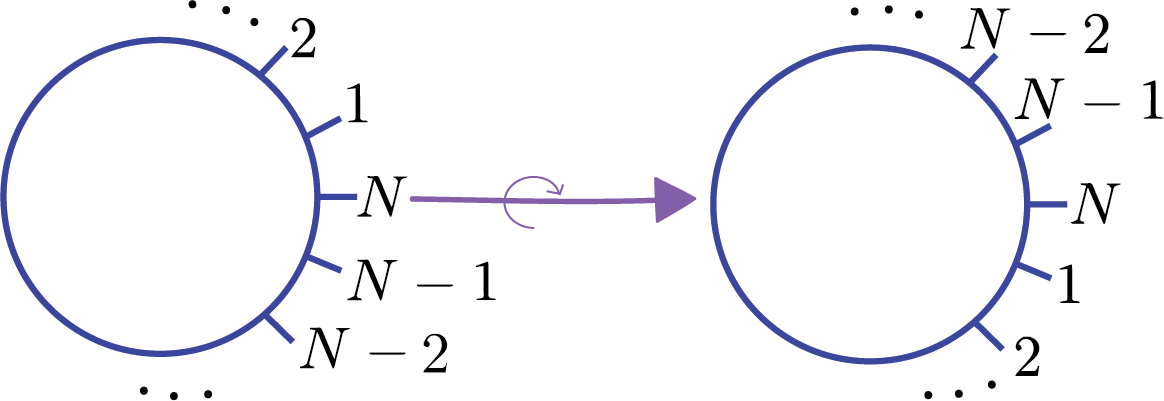
\includegraphics[width=0.6\textwidth]{Figures/Reflection_over_circle.png}
    \caption{Meaning of the relabel done in the circulant matrix, which can be seen as a reflection over the circle.}
    \label{reflectioncircle}
\end{figure}
Explicitly we can write that if $\tilde{\Gamma}^{+}_{mn}$ has the shape
\begin{equation}
\left(\begin{array}{ccccc}
a_{0} & a_{-1} & \cdots & a_{2} & a_{1} \\
a_{1} & a_{0} & \cdots & a_{3} & a_{2} \\
\cdot & \cdot & \cdot & \cdots & \cdot \\
\vdots & \vdots & \vdots & \vdots & \vdots \\
a_{-1} & a_{-2} & a_{-3} & \cdots & a_{0}
\end{array}\right),
\end{equation}
then $\tilde{\Gamma}^{-}_{mn}$ will be given by
\begin{equation}
\left(\begin{array}{ccccc}
a_{0} & a_{1} & \cdots & a_{-2} & a_{-1} \\
a_{1} & a_{2} & \cdots & a_{-1} & a_{0} \\
\cdot & \cdot & \cdot & \cdots & \cdot \\
\vdots & \vdots & \vdots & \vdots & \vdots \\
a_{-1} & a_{0} & a_{1} & \cdots & a_{-2}
\end{array}\right),
\end{equation}
which we name anticirculant.\\
\indent In this way, both the circulant and the anticirculant parts of $\Gamma$ are computed as Fourier transforms of the vectors $m^{+}(\theta_k)e^{i\phi(\theta_k)}$ and $m^{-}(\theta_k)e^{i\phi(\theta_k)}$ respectively.\\
\indent Here we spot 3 things. First, the FCM always can be written as a circulant matrix $\Gamma^{+}$ plus an anticirculant matrix $\Gamma^{-}$. Second, in the ground state, the FCM is circulant because the fermion occupation numbers $n^{c}\left(\theta_{k}\right)=n^{s}\left(\theta_{k}\right)=0, \forall k$. Third, for a generic excited state, we have that in average the FCM matrix is always circulant, because $\langle n^{c}\left(\theta_{k}\right)\rangle=\langle n^{s}\left(\theta_{k}\right)\rangle$.
\subsection{Local modes in the fermionic chains}
For our purpose, it is important to study the behaviour of reduced states in the chain, that is, we want to look into small portions of size $L$ in a translationally invariant chain of size $N$ ($N>L$). To do this it is convenient to write the modes of the small chain of size $L$ in terms of the modes of whole chain of size $N$.\\
\indent Since we work with a one-dimensional, translationally invariant closed chain of $N$ free fermions, with local interactions, it is often useful to expand the annihilation/creation operators $\hat{a}_x$ ($\hat{a}^{\dagger}_l$) at the site $x$ ($x = 0,1,\ldots, N-1$) in terms of their counterpart in the plane-wave basis, obtained through
\begin{equation}
\hat{b}_{q} = \frac{e^{i\eta_q}}{\sqrt{N}}\sum_{x=0}^{N-1}e^{-i\theta_q x}\hat{a}_x,
\end{equation}
and its hermitian conjugate, with $\theta_q = \frac{2\pi}{N}q$, and $\eta_q$ is a phase to be adjusted. By doing so, we showed that in the case of the $XY$ model, the Hamiltonian \eqref{CH2:Hamiltonian_jordan_wigner} became diagonal on the operators $\hat{b}_q$, explicitly we showed that the Hamiltonian had the form
\begin{equation}
\hat{H} = \sum_{q=0}^{N} \Lambda(\theta_q)\hat{b}_q^{\dagger}\hat{b}_q,
\label{CH2:Hamiltonian_diagonal}
\end{equation}
with $\Lambda(\theta_q)$ given by \eqref{CH3:Spectrum_XY_model} in the $XY$ model.\\
\indent We consider now a set of local plane wave modes for the portion of the chain of length $L$ comprising the sites $x=0,1,\ldots,L-1$,
\begin{equation}
\tilde{b}_k = (-1)^{k}\frac{e^{-i\tilde{\theta_k}/2}}{\sqrt{L}}\sum_{x=0}^{L-1}e^{-i\tilde{\theta}_k x}\hat{a}_x,
\end{equation}
where similarly as in the case of the large chain of size $N$, we take $\tilde{\theta}_k = \frac{2\pi}{L}k$. By introducing the modes of the local chain in this way, the plain wave modes will diagonalize any Hamiltonian of the form \eqref{CH2:Hamiltonian_diagonal}, with $N$ replaced by $L$.\\
\indent We now expand the local operators $\tilde{b}_k$ in terms of the global operators $\hat{b}_q$ that are defined over the chain of size $N$. The relation between the two becomes
\begin{equation}
\tilde{b}_k = \frac{1}{\sqrt{NL}}\sum_{q=0}^{N-1} D_{L}(\theta_q-\tilde{\theta}_k) \hat{b}_q,
\label{CH2:From_L_to_N}
\end{equation}
where we chose appropriately  $\eta_q = \theta_q(L-1)/2$, and
\begin{equation}
D_{L}(\theta) = \frac{\sin\left(\frac{\theta}{2}L\right) }{\sin\left(\frac{\theta}{2}\right)},
\end{equation}
is the Dirichlet kernel\cite{bashirov_chapter_2014}.\\
\indent Now consider an excited state $\ket{\vec{n}}$ of the chain, described by a set of excitation numbers $\vec{n}\equiv (n_0,n_1,\ldots, n_{N-1})$, where $n_q\in \{0,1\}$. In particular the state satisfies
\begin{equation}
\bra{\vec{n}}\hat{b}^{\dagger}_{q}\hat{b}_{q'}\ket{\vec{n}} = \delta_{q,q'}n_q,\quad \bra{\vec{n}}\hat{b}_{q}\hat{b}_{q'}\ket{\vec{n}} = \bra{\vec{n}}\hat{b}^{\dagger}_{q}\hat{b}^{\dagger}_{q'}\ket{\vec{n}} = 0,
\end{equation}
for all $q,q'$. To any excited state, we can associate the correspondent $L\times L$ FCM, that is
\begin{equation}
A_{kk'}(\vec{n}) = \bra{\vec{n}}\tilde{b}^{\dagger}_k \tilde{b}_{k'}\ket{\vec{n}} = \frac{1}{NL}\sum_{q=0}^{N-1}D_{L}(\theta_q-\tilde{\theta}_k)D_L(\theta_q-\tilde{\theta}_{k'})n_q.
\end{equation}
Therefore, we have a full characterization of any subchain in the state $\ket{\vec{n}}$, or equivalently in the state
\begin{equation}
\rho_L(\vec{n}) = \operatorname{Tr}_{N-L} \ket{\vec{n}}\bra{\vec{n}},
\end{equation}
the corresponding partial density matrix on the subchain.
\section{Error correcting code theory}
\begin{figure}[H]
\centering
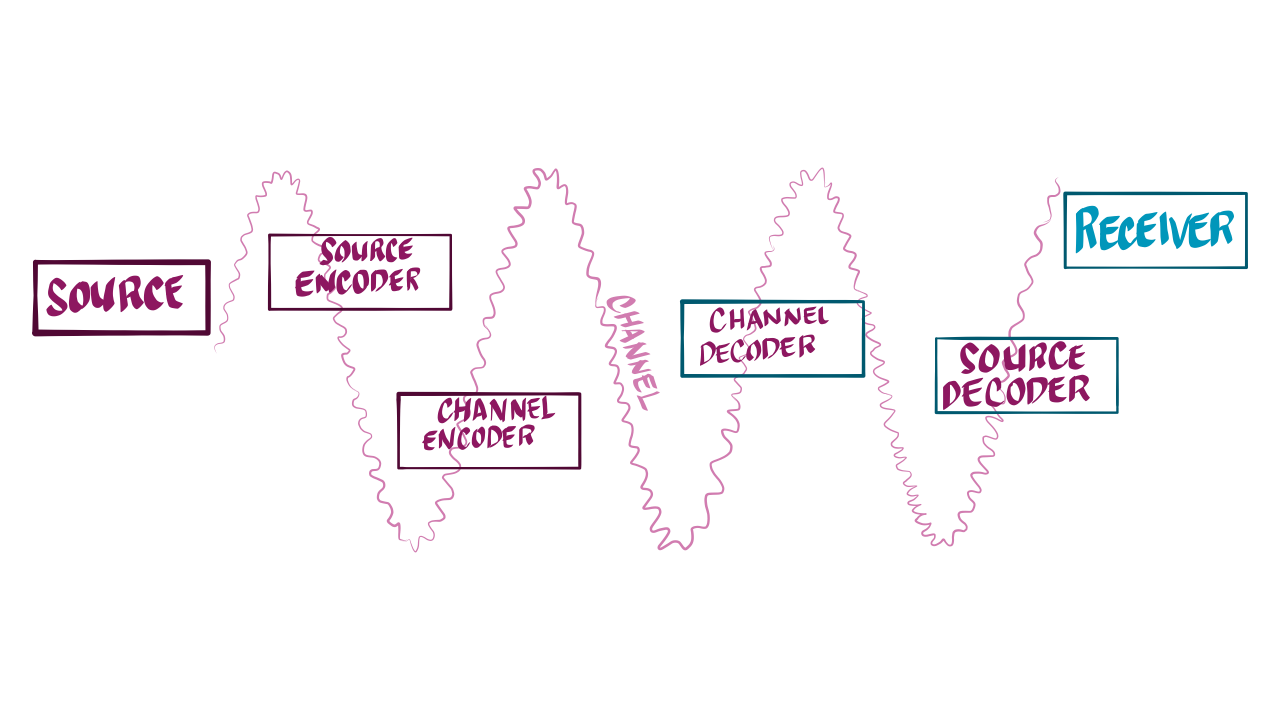
\includegraphics[width=0.7\textwidth]{Figures/Source_Destination.png}
\caption{Representation of the scheme of communication.The encoding system introduces some redundancy into the transmitted vector $\mathbf{x}$. The decoding system uses this known redundancy to deduce from the received vector $\mathbf{y}$ both the original source vector and the noise introduced by the channel.}
\label{CH2:Channel_communication}
\end{figure}
We will now turn to study error correcting codes. We start by motivating the problem of error correction codes as a mechanism to understand communication, then we move to introduce basic definitions to formalise the problem of error correcting codes, and afterwards, we will move to study the case of random minimum distance codes and some interesting results about them.\\

\indent Every day we communicate over noisy channels such as in telephone lines, over which two devices communicate digital information through a bunch of cables. When we think in designing these channels we have as main purpose to be able to transmit information in a reliable way while dealing with  errors induced by the noise in the channel. Information theory and coding theory offer a way to study communications as C. Shannon pointed out in $1948$ \cite{shannon_mathematical_1948}. In order to stablish communication, there are some main ingredients that C. Shannon explicitly presented in his paper \cite{shannon_mathematical_1948}.\\
\indent As we illustrate in figure \ref{CH2:Channel_communication} in order to pass a message through a channel to then someone receive it, we add encoders before the channel and decoders after it. The encoders encode the source message $\mathbf{x}$ into a transmitted message $\mathbf{y}$, adding redundancy to the original message in some way. The channel adds noise to the transmitted message, yielding a received message $\mathbf{y}$. The decoders use the known redundancy introduced by the encoding system to infer both the original signal $\mathbf{s}$ and the added noise.
\subsection{Channel coding}
\begin{figure}[H]
\centering
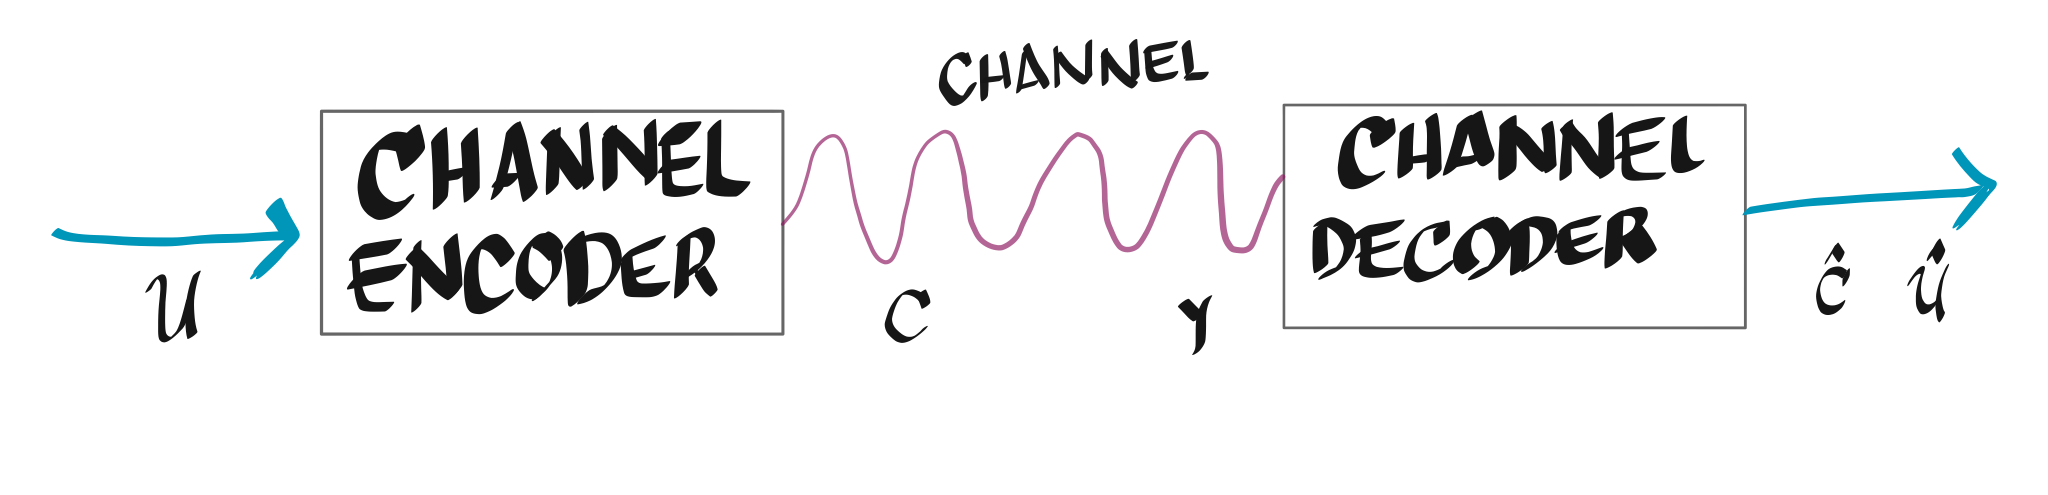
\includegraphics[width=0.8\textwidth]{Figures/Channel_decoder.png}
\caption{Channel coding}
\label{CH2:Channel_communication_2}
\end{figure}
For the purpose of our work, the model of channel we will use, is the \textit{discrete probability channel}: a probabilistic channel $S$ is defined as a triple $(F,\Phi,\operatorname{Prob})$, where $F$ is a finite \textit{input alphabet}, $\Phi$ is a finite \textit{output alphabet}, and $\operatorname{Prob}$ is a conditional probability distribution
\begin{equation}
\operatorname{Prob}\{\mathbf{y}\text{ received }|\mathbf{x}\text{ transmited}\},
\end{equation}
defined for every pair $(\mathbf{x},\mathbf{y})\in F^{m}\times\Phi^m$, where $m$ ranges over all positive integers and $F^m/\Phi^m$ denotes the set of all words of length $m$ over $F/\Phi$. It is important to clarify that we assume that the channel neither deletes nor inserts symbols; that is, the length of the output word $\mathbf{y}$ always equals the length of the input word $\mathbf{x}$.\\
\indent The input channel encoder is an \textit{information word} $\mathbf{u}$ out of $M$ possible information words (see figure \ref{CH2:Channel_communication_2}). The channel encoder generates a \textit{codeword} $\mathbf{c}\in F^n$ that is input to the channel. The resulting output of the channel is a received word $\mathbf{y}\in\Phi^n$, which is fed into the channel decoder. the decoder, in turn, produces a \textit{decoded codeword} $\hat{\mathbf{c}}$ and a \textit{decoded information word} $\hat{\mathbf{u}}$, with the aim of having $\mathbf{c}=\hat{\mathbf{c}}$ and $\mathbf{u}=\hat{\mathbf{u}}$. this implies that the channel encoder needs to be such that the mapping $\mathbf{u}\mapsto \mathbf{c}$ is one to one.
\begin{definition}[Rate \cite{roth_2006}]
The \textit{rate} of the channel encoder is defined as 
\begin{equation}
R = \frac{\log_{|F|}M}{n}.
\end{equation}
\end{definition}
If all information words have the same length over $F$, then this length is given by the numerator, $\log_{|F|}M$, in the expression for $R$. Since the mapping of the encoder is one-to-one, we have that $R\leq 1$.\\
In the case where the input alphabet $F$ has the same size as the output alphabet $\Phi$, it will be convenient to assume that $F=\Phi$ and that the elements of $F$ form a finite Abelian group. We then say that the channel is an \textit{additive channel}.\\
\indent Given an additive channel, let $\mathbf{x}$ and $\mathbf{y}$ be input and output words, respectively, both in $F^m$. the \textit{error word} is defined as the difference $\mathbf{x}-\mathbf{y}$, where the subtraction is taken component by component. The action of the channel can be described as adding an error word $\mathbf{e}\in F^m$ to the input word $\mathbf{x}$ to produce the output word $\mathbf{y} = \mathbf{x}+\mathbf{e}$.\\
\indent When $F$ is an Abelian group, it contains the zero (or unit) element. The \textit{error locations} are indexes of the nonzero entries in the error word $\mathbf{e}$. Those entries are referred to as the \textit{error values}\cite{roth_2006}\footnote{Taken from \cite{roth_2006}}.
\subsection{Binary symmetric channel (BSC)}
We consider as an example of the previous definitions the input and output alphabets are $F=\Phi=\{0,1\}$, and for every two binary words $\mathbf{x}$, $\mathbf{y}$ for a given length $m$, 
\begin{align}
\operatorname{Prob}\{\mathbf{y}\text{ received }|\mathbf{x}&\text{ transmited}\} \nonumber \\
&=\prod_{j=1}^{m} \operatorname{Prob}\{y_j\text{ received }|x_j\text{ transmited}\},
\end{align}
where for every $x,y\in F$,
\begin{equation}
\operatorname{Prob}\{y\text{ received }|x\text{ transmited}\} = \left\{
    \begin{array}{ll}
        1-p & \mbox{if } y=x \\
        p & \mbox{if } y\neq x
    \end{array}
\right.
\end{equation}
The parameter $p$ is a real number $0\leq p\leq 1$  is called the \textit{crossover probability} of the channel.\\
\indent the action of the BSC can be described as flipping each input bit with probability $p$, independently of the past or the future. The channel is called symmetric since the probability of the flip is the same regardless of weather the input is $0$ or $1$.
\subsection{Block codes}
An $(n,M)$ (\textit{block}) code over a finite alphabet $F$ is a nonepty subset $\mathfrak{C}$ of size $M$ of $F^n$. The parameter $n$ is called the \textit{code length} and $M$ is the \textit{code size}\cite{roth_2006}. The \textit{information length} or \textit{codeword length} of $\mathfrak{C}$ is defined by $k=\log_{|F|}M$, and the \textit{rate} is $R=k/n$. The range of the mapping defined by the channel encoder in figure \ref{CH2:Channel_communication_2} forms an (n,M) code, and this in which the term $(n,M)$ code will be used. The elements of a code are called \textit{codewords}\cite{roth_2006}.\\
\indent In addition to the length and size of a code, we will be interested in quantifying how much the codewords in the code differ from each other. To do this, we will introduce the following definitions.
\begin{definition}[Hamming distance \cite{roth_2006}]
Let $F$ be an alphabet. The Hamming distance between two codewords $\mathbf{x},\mathbf{y}\in F^n$ is the number of coordinates on which $\mathbf{x}$ and $\mathbf{y}$ differ. the Hamming distance will be denoted by $d(\mathbf{x},\mathbf{y})$.
\end{definition}
\indent It is easy to verify that the Hamming distance satisfies the following properties of a metric for every three words $\mathbf{x},\mathbf{y},\mathbf{z}\in F^n$.
\begin{enumerate}[label=(\roman*)]
\item $d(\mathbf{x},\mathbf{y})\geq 0$, with equality if and only if $\mathbf{x}=\mathbf{y})$.
\item Symmetry: $d(\mathbf{x},\mathbf{y})=d(\mathbf{y},\mathbf{x})$.
\item The triangle inequality: $d(\mathbf{x},\mathbf{y}) \leq d(\mathbf{x},\mathbf{z})+ d(\mathbf{z},\mathbf{y})$.
\end{enumerate}
\begin{definition}[Hamming weight \cite{roth_2006}]
Let $F$ be an Abelian group. The Hamming weight of $\mathbf{e}\in F^n$ is the number of nonzero entries in $\mathbf{e}$. We denote the Hamming weight by $w(\mathbf{e})$.
\end{definition}
\indent Notice that for every two words $\mathbf{x}, \mathbf{y}\in F^n$,
\begin{equation}
d(\mathbf{x},\mathbf{y}) = w(\mathbf{y}-\mathbf{x}).
\end{equation}
Turning back now to block codes, let $\mathfrak{C}$ be an $(n,M)$ code over $F$ with $M>1$. The \textit{minimum distance} of $\mathfrak{C}$ is the minimum Hamming distance between any two distinct codewords of $\mathfrak{C}$; that is, the minimum distance $d$ is given by
\begin{equation}
d=\min_{\mathbf{c}_1,\mathbf{c}_2\in \mathfrak{C} : \mathbf{c}_1\neq \mathbf{c}_2} d(\mathbf{c}_1,\mathbf{c}_2).
\end{equation}
An $(n,M)$ with minimum distance $d$ is often called $(n,M,d)$ code. We will sometimes use the notation $d(\mathfrak{C})$ for the minimum distance of a given code $C$.
\subsection{Decoding}
Let $\mathfrak{C}$ be an $(n,M,d)$ code over an alphabet $F$ and let $S$ be the channel defined by the triple $(F,\Phi,\operatorname{Prob})$. A decoder for the code $\mathfrak{C}$with respect to the channel $S$ is a function
\begin{equation}
\mathcal{D}: \Phi^n\to \mathfrak{C}.
\end{equation}
The \textit{decoding error probability} $P_{\text{err}}$ of $\mathcal{D}$ is defined by
\begin{equation}
P_{\text{err}} = \max_{\mathbf{c}\in\mathfrak{C}} P_{\text{err}}(\mathbf{c}),
\end{equation}
where 
\begin{equation}
P_{\text{err}}(\mathbf{c}) = \sum_{\mathbf{y}:\mathcal{D}(\mathbf{y})\neq \mathbf{c}} \operatorname{Prob}\{\mathbf{y}\text{ received }|\mathbf{c}\text{ transmited}\}.
\end{equation}
Note that $P_{\text{err}}(\mathbf{c}$ is the probability that the code word $\mathbf{c}$ will be decoded erroneously, given that $\mathbf{c}$ was transmitted.
\subsubsection*{Maximum-likelihood decoding}
Consider particular strategies for codes and channels. Given an $(n,M,d)$ code $\mathfrak{C}$ over $F$ and a channel $S = (F,\Phi,\operatorname{Prob})$, a \textit{maximum-likelihood decoder} (MLD) for $\mathfrak{C}$ with respect to $S$ is the function $\mathcal{D}_{MLD}:\Phi^n\to \mathfrak{C}$ defined as follows: for every $\mathbf{y}\in \Phi^n$, the value  $\mathcal{D}_{MLD}$ equals the codeword $\mathbf{c}\in\mathfrak{C}$ that maximizes the probability
\begin{equation}
\operatorname{Prob}\{\mathbf{y}\text{ received }|\mathbf{c}\text{ transmited}\},
\end{equation}
In the case of a tie between two (or more) codewords, we choose one of the tying codewords arbitrarily. Hence, $\mathcal{D}_{MLD}$ is well-defined for the code $\mathfrak{C}$ and the channel S.
\subsubsection*{Decoder in repetition code}
As an alternative to the MLD we will consider a \textit{majority vote decoder},  we consider $\mathfrak{C}$ to be the binary $(3,2,3)$ \textit{repetition code} and let $S$ be the BSC with crossover probability $p$.\\
\indent The binary $(3,2,3)$ repetition code is the code $\{000,111\}$ over $F=\{0,1\}$, which has information length $\log_2 2=1$ and rate $1/3$.\\
Define a decoder $\mathcal{D}:\{0,1\}^3\to \mathfrak{C}$ as follows:
\begin{equation}
\mathcal{D}(000)=\mathcal{D}(001)=\mathcal{D}(010)=\mathcal{D}(100) = 000,
\end{equation}
and
\begin{equation}
\mathcal{D}(011)=\mathcal{D}(101)=\mathcal{D}(110)=\mathcal{D}(111) = 111.
\end{equation}
This decoder is known as the vote majority decoder.\\
\indent The probability $P_{\text{err}}$ equals the probability of having two or more errors \cite{roth_2006}
\begin{align}
P_{\text{err}} = P_{\text{err}}(000) = P_{\text{err}}(111) &= {3 \choose 2}p^2(1-p) + {3 \choose 3}p^3\nonumber\\
&=3p^2-3p^3+p^3\nonumber\\
&=3p^2-2p^3.
\label{CH2:majority_vote}
\end{align}
Notice then that the error probability is dominated by the probability that two bits in a block of tree are flipped, which scales as $p^2$. Since our goal is to have decoders with small $P_{\text{err}}$, from equation \eqref{CH2:majority_vote} we conclude that $P_{\text{err}}$ is smaller than $p$ when $p<1/2$, which simply means that coding has improved the probability of error per message, compared to uncoded transmission. However, the price is reflected in the rate: three bits are transmitted for every bit implies a rate of $\log_2 M/n = 1/3$.
\subsubsection*{Nearest-codeword decoder}
\indent We next consider a particular decoding strategy. A \textit{nearest-codeword decoder} for an $(n,M)$ code $\mathfrak{C}$ over $F$ is a function $F^n\to \mathfrak{C}$ whose value for every word $\mathbf{y}\in F^n$ is a closes codeword in $\mathfrak{C}$ to $\mathbf{y}$, where the term ``closest'' is with respect to the Hamming distance. A nearest-codeword decoder for $\mathfrak{C}$ is a decoder for $\mathfrak{C}$ with respect to any additive channel whose input and output alphabets are $F$.
\subsubsection{Capacity of the binary symmetric channel}
So far we have seen that coding allows to reduce the decoding error probability $P_{\text{err}}$, at the expense of transmitting at lower rates. As we will discuss, it is possible to achieve arbitrarily small values of $P_{\text{err}}$, while still transmitting at rates that are bounded away from $0$.\\
\indent The \textit{binary entropy} function $\mathfrak{H}:[0,1]\to[0,1]$ is defined by
\begin{equation}
\mathfrak{H}(x) = -x\log_2 x-(1-x)\log_2 (1-x),
\label{CH2:Binary entropy}
\end{equation}
where $\mathfrak{H}(0)=\mathfrak{H}(1)=0$.\\
\indent Now let $S$ be the BSC with crossover probability $p$. The \textit{capacity} of $S$ is given by
\begin{equation}
\operatorname{Cap}(S) = 1-\mathfrak{H}(p).
\end{equation}
These definitions will allows us to present a special case of two fundamental results in information theory. These results state the the capacity of a channel is the largest rate at which information can be transmitted reliably through that channel
\begin{theorem}[Shannon coding theorem for the BSC]
Let s be the BSC with crossover probability $p$ and let $R$ be a real in the range $0\leq R \leq \operatorname{Cap}(S)$. there exist an infinite sequence of $(n_i,M_i)$ block codes over $F\{0,1\}$, $i=1,2,\ldots$, such that $(\log_2 M_i)/n_i\geq R$ and, for maximum-likelihood decoding for those codes (with respect to S), the decoding error probability $P_{\text{err}}$ approaches $0$ as $i\to \infty$.
\end{theorem}
\begin{theorem}[Shannon converse coding theorem for the BSC \cite{roth_2006}] Let $S$ be the BSC channel with crossover probability $p$ and let $R$ be a real greater than $\operatorname{Cap}(S)$. Consider any infinite sequence of $(n_i,M_i)$ block codes over $F=\{0,1\}, i = 1,2,\ldots$, such that $(\log_2 M_i)/n_i\geq R$ and $n_1< n_2<\cdots< n_i < \cdots$. Then, for any decoding scheme for those codes (with respect to S), the decoding error probability $P_{\text{err}}$ approaches $1$ as $i\to \infty$.
\end{theorem}
These theorems are know as the noisy-channel theorems for the special case of the BSC. A problem with announcing the theorems in this particular way is that are quite general results; meaning that the theorems only says that reliable communication with crossover probability $p$ and rate $R$ can be achieved by using code blocks with sufficiently large code length $n_i$\footnote{To see further details about the proof see \cite{mackay_information_2003, roth_2006} and \textbf{explicitly} taken from \cite{roth_2006}}. The theorem does not say how large $n$ needs to be to achieve given values of $R$ and $p$. Particularly, it is possible to show that $P_{\text{err}}$ in these theorems can be guaranteed to decrease exponentially with the code length $n_i$.\\
\indent For a discrete memoryless channel, a length code $n$ and rate $R$, there exist a block code $(n,M)$ whose average probability of error satisfies:

\begin{equation}
P_{\text{err}}\leq \operatorname{exp}(-n E_{r}(R)),
\label{CH2:randomexpoenent}
\end{equation}
where $E_r(R)$ is known as the \textit{random-coding exponent} of the channel, a convex, decreasing, positive function of $R$ for $0\leq R\leq \operatorname{Cap}(S)$. the random-coding exponent is also known as the reliability function \cite{gallager_information_1968, gallager_random_2006}. $E_r(R)$ approaches zero as $R\to  \operatorname{Cap}(S)$. As we will see the computation of the random-coding exponent is in general a challenging task on which much effort has been expended.


\subsection{Levels of error handling}
While the setting in previous sections was probabilistic, we will move to identify error words that are generated by an additive channel and are always recoverable, as long as the transmitted codewords are taken from a block code whose minimum distance is sufficiently large. The results we present here are combinatorial, meaning that they do not depend on the particular conditional probability of the channel.

\subsection{Random minimum distance codes and its error exponents}
Having in mind that for minimum distance codes it is possible to perfectly recover the message up to a number of error of $\lfloor(d-1)/2\rfloor$, we will study the case of random minimum distance codes over the memoryless binary channel with crossover probability $p=1/2$.\\
\indent Let  $\mathfrak{C}$ be a random block code $(n,M\equiv 2^{nR})$ over $F= \{0,1\}$ and rate $R$. This is known as a random code ensemble (RCE) and is obtained by uniformly random choosing each of the $n$ bits in each of the $M$ codewords independently. Equivalently, each of the $2^{nM}$ possible binary codes of length $n$ and rate $R$ in the RCE is assigned probability $2^{-nM}$.\\
\indent Since these codes are randomly chosen we can ask ourselves if these codes will have minimum distance and if so we will be interested in the distribution of distances. To answer this, we first compute the probability that a given random codeword $\mathbf{x}_i$  of length $n$ will be at a Hamming distance $d=\delta n$ from an arbitrary binary $n$-tuple $\mathbf{y}$, where $\delta=d/n$ is known as the \textit{relative distance}. This probability is independent of $\mathbf{y}$ and equals \cite{barg_random_2002}
\begin{equation}
\operatorname{Prob}(d(\mathbf{x}_i,\mathbf{y})=d) = {n \choose d}\left(\frac{1}{2} \right)^{d} \left( \frac{1}{2}\right)^{n-d} \equiv 2^{-n(1-\mathfrak{H}(\delta))},
\label{CH2:probability_of_having}
\end{equation}
where $\mathfrak{H}(\delta)$ is the binary entropy defined in \eqref{CH2:Binary entropy}. Under this RCE, two Hamming distances $d(\mathbf{x}_i,\mathbf{x}_j)$, $d(\mathbf{x}_i',\mathbf{x}_j')$ are independent random variables unless $\{i,j\} = \{i',j'\}$ or $\{i,j\}= \{j',i'\}$.\\
\indent Consider the number of unordered pairs of codewords $(\mathbf{x}_i,\mathbf{x}_j)$ with $i\neq j$ in $\mathfrak{C}$ at Hamming distance $d$ apart
\begin{equation}
\mathcal{S}_{\mathfrak{C}}(d) = \sum_{i=0}^{M-1}\sum_{j=0}^{i-1} \Theta\{d(\mathbf{x}_i,\mathbf{x}_j) = d\},
\end{equation}
where $\Theta\{d(\mathbf{x}_i,\mathbf{x}_j) = d\}$ is the indicator of the event in the brackets, that is, $\Theta\{d(\mathbf{x}_i,\mathbf{x}_j) = d\}$ is equal to $1$ if $d(\mathbf{x}_i,\mathbf{x}_j) = d$ and to $0$ otherwise. Then $\mathcal{S}_{\mathfrak{C}}(d)$ is a sum of ${M \choose 2}$ pairwise-independent, identically distributed random variables $\Theta\{d(\mathbf{x}_i,\mathbf{x}_j) = d\}$, each with mean
\begin{equation}
\mathbb{E}\Theta = \operatorname{Prob}\{d(\mathbf{x}_i,\mathbf{x}_j) = d\},
\end{equation}
where $\mathbb{E}$ refers to the expected value or simply the average of a random variable which is obtained by
\begin{equation}
\mathbb{E}(X) = \sum_{x\in X} \operatorname{Prob}(X=x) x,
\end{equation}
with $X$ a random variable.\\
The variance of $\Theta\{d(\mathbf{x}_i,\mathbf{x}_j) = d\}$ is
\begin{equation}
\operatorname{Var}[\Theta] = \mathbb{E}\Theta^2 - (\mathbb{E}\Theta)^2 = \mathbb{E}\Theta - (\mathbb{E}\Theta)^2 <  \mathbb{E}\Theta,
\end{equation}
where we have used the fact that $\Theta^2 = \Theta$ since $\Theta$ is a $\{0,1\}$-valued function. We have then that in the case of the BSC, $\mathcal{S}_{\mathfrak{C}}(d)$ is a sum of ${M \choose 2}$ independent and identically distributed random variables.
\begin{equation}
\mathbb{E}\mathcal{S}_{\mathfrak{C}}(d) = {M\choose 2} \mathbb{E}\Theta = 2^{n(2R-1+\mathfrak{H}(\delta))},
\label{CH2:average_number_codes}
\end{equation}
where we have used the fact that $M \sim 2^{nR}$, ${M \choose 2}=M(M-1)/2\sim M^2=2^{2nR}$. Since the variance of a sum of uncorrelated random variables is equal to the sum of their variances
\begin{equation}
\operatorname{Var}(\mathcal{S}_{\mathfrak{C}}(d)) = {M \choose 2} \operatorname{Var}\Theta < \mathbb{E} \mathcal{S}_{\mathfrak{C}}(d).
\end{equation}
As we mentioned before, we will be interested in study the minimum distance $d(\mathfrak{C})$ that this particular kind of codes have. To do this we first announce the next three lemmas that will let us introduce one of the main results in \cite{barg_random_2002} about the distribution of minimum distance in random codes.


\begin{lemma}[Markov inequality]
Let $X$ be a non-negative real random variable, and $\alpha >0$, then the probability that $X$ is at least $\alpha$ is at most the expectation of $X$ divided by $\alpha$,
\begin{equation}
\operatorname{Prob}(X\geq \alpha)\leq \frac{\mathbb{E}(X)}{\alpha}
\end{equation}
\end{lemma}

\begin{lemma}[Chebyshev's inequality]
Let $X$ be real random variable with finite expected value $\mathbb{E}(X)=\mu$ and finite variance $\operatorname{Var}(X) = \sigma^2$, then for all $k >0$,
\begin{equation}
\operatorname{Prob}(|X-\mu|\geq k)\leq \frac{\sigma^2}{k^2}
\end{equation}
\end{lemma}

\begin{proof}
Apply Markov's inequality with $\alpha \equiv k^2$ and take the random variable $X-\mu$
\begin{equation}
\operatorname{Prob}\left((X-\mu)^2\geq k^2\right)\leq \frac{\mathbb{E}(X-\sigma)}{k^2} = \frac{\sigma^2}{k^2}
\end{equation}
\end{proof}

\begin{lemma}[Chernoff bound]
Let $X$ be real random variable with finite mean, for all $\alpha>0$ and $t>0$,
\begin{equation}
\operatorname{Prob}(X\geq \alpha)\leq \frac{\mathbb{E}(e^{t X})}{e^{t\alpha }}
\label{CH2_chernoff_bound}
\end{equation}
\end{lemma}
\begin{proof}
First, take the exponential at both sides of the expression $\operatorname{Prob}(X\geq \alpha)$,
\begin{equation}
\operatorname{Prob}(X\geq \alpha) = \operatorname{Prob}(e^{tX}\geq e^{t\alpha}),
\label{CH2:proof_chernoff_bound}
\end{equation}
then we apply Markov's inequality and conclude that
\begin{equation}
\operatorname{Prob}(X\geq \alpha)= \operatorname{Prob}(e^{tX}\geq e^{t\alpha})\leq \frac{\mathbb{E}(e^{t X})}{e^{t\alpha }}
\end{equation}
\end{proof}
In particular, we can optimize over $t$ to get
 \begin{equation}
\operatorname{Prob}(X\geq \alpha)\leq \min_{t>0} \frac{\mathbb{E}(e^{t X})}{e^{t\alpha }}.
\label{CH2:optimal_chernoff_bound}
\end{equation}
Now we are ready to state the the following theorem\cite{barg_random_2002}.

\begin{theorem}[Distance distribution in RCE]
For $0\leq R< 1/2$ and any $\varepsilon>0$, the probability that a code length $n$ and rate $R$ from the RCE has relative minimum distance less than $\delta_{GV}(2R)-\varepsilon$, with $\delta_{GV}(R) $ the solution to the equation $\mathfrak{H}(\delta) = 1-R$, goes to zero exponentially as $n\to \infty$. For $0\leq R < 1$, if $d=n\delta$ is such that
\begin{equation}
\delta_{GV}(2R)+\varepsilon \leq \delta \leq 1- \delta{GV}(2R) - \varepsilon,
\end{equation}
then the probability that the number of codeword pairs at a distance d satisfies $\mathcal{S}_{\mathfrak{C}}(d) \doteq 2^{n(2 R-1+\mathfrak{H}(\delta))}$ goes to one as $n\to \infty$.
\end{theorem}

\begin{proof}
For a given value of the code value of the code rate $R$ we can choose $d$ such that $d/n\to\delta \leq \delta_{\mathrm{GV}}(2 R)-\varepsilon$. Then
\begin{equation}
\operatorname{Prob}\left\{\mathcal{S}_{\mathfrak{C}}(d) \geq 1\right\} \leq \mathbb{E} \mathcal{S}_{\mathfrak{C}}(d) \doteq 2^{-n(1-\mathfrak{H}(\delta)-2 R)} \rightarrow 0,
\end{equation}
which in other words it tells us that with probability differing from $1$ by an exponentially falling quantity, there will be no pairs at distance $d$. Conversely, if $\delta_{\mathrm{GV}}(2 R)+\varepsilon<\delta<1-\delta_{\mathrm{GV}}(2 R)-\varepsilon$, then $1-\mathcal{H}(\delta)<2R$ and the average of number of pairs $\mathbb{E} \mathcal{S}_{\mathfrak{C}}(d))$ at a distance $d$ is exponentially large. To see this, we can use the Chebyshev's inequality, so for any $\delta>0$, we have 
\begin{equation}
\operatorname{Prob}\left\{\left|\mathcal{S}_{\mathfrak{C}}(d)-\mathbb{E} \mathcal{S}_{\mathfrak{C}}(d)\right| \geq\left(\begin{array}{c}
M \\
2
\end{array}\right) \alpha\right\} \leq \frac{\mathbb{E} \Theta}{\left(\begin{array}{c}
M \\
2
\end{array}\right) \alpha^{2}},
\end{equation}
by choosing $\alpha \doteq 2^{-n(1-\mathfrak{H}(\delta)+\Delta)}<\mathbb{E} \Theta$ for any $\Delta>0$, then we have
\begin{equation}
\operatorname{Prob}\left\{\left|\mathcal{S}_{\mathfrak{C}}(d)-\mathbb{E}\mathcal{S}_{\mathfrak{C}}(d)\right|>\left(\begin{array}{c}
M \\
2
\end{array}\right) \alpha\right\}\leq \frac{2 \mathbb{E} \Theta}{M(M-1) \alpha^{2}} \doteq 2^{-n(2 R-1+\mathfrak{H}(\delta)-2 \Delta)}.
\label{CH2:probability_result}
\end{equation}
The exponent on the right-hand side can be made positive by choosing $\Delta$ small enough. This establishes the fact that $\mathcal{S}_{\mathfrak{C}}(d)\doteq 2^{n(2 R-1+\mathcal{H}(\delta))}$ for the chosen value of $d$ with probability tending to one as $n\to\infty$.
\end{proof}
Alternative this result can be expressed as follows. With probability $1-2^{-\zeta(n)}$ as $n\to \infty$, the relative minimum distance of a code drawn from the RCE will be approximately $\delta{GV}_(2R)$ for $0\leq R \leq \frac{1}{2}$ and $0$ for $\frac{1}{2}\leq R\leq 1$.\\
\indent Define the distance distribution the random code $\mathfrak{C}$ as
\begin{equation}
\mathcal{N}_{\mathfrak{C}}(d)  = \frac{2}{M} \mathcal{S}_{\mathfrak{C}}(d), \quad  (d=0,1,\ldots , n).
\end{equation}
Thus $\mathcal{N}_{\mathfrak{C}}(d)$ is the average over the $M$ codewords $\mathbf{x}_i$ of the number of other codewords $\mathbf{x}_j, j \neq i$, at Hamming distance $d$ from $\mathbf{x}_i$.
\indent We therefore have shown that the complete average distance distribution over RCE is
\begin{equation}
\mathcal{N}_{RCE}(d)  = \frac{2}{M} \mathbb{E} \mathcal{S}_{\mathfrak{C}}(d) \doteq 2^{n(R-1+\mathfrak{H}(\delta))}.
\end{equation}
Since the probability in \eqref{CH2:probability_result} tends to zero exponentially and since there are only $N+1$ different values of distance $d$, theorem $2.5.7$ implies that for almost all codes in RCE $\mathcal{N}_{\mathfrak{C}}(d) \doteq \mathcal{N}_{RCE}(d)$ for all $d$ such that $\delta_{\mathrm{GV}}(2 R)+\varepsilon \leq \delta \leq 1-\delta_{\mathrm{GV}}(2 R)-\varepsilon$. However for $\delta \leq \delta_{\mathrm{GV}}(2 R)-\varepsilon$ or $\delta \geq 1-\delta_{\mathrm{GV}}(2 R)+\varepsilon$, the $\mathcal{N}_{RCE}(d)=0$.\\


In the next chapter, we will develop the correspondent connection between systems whose Hamiltonians are quadratic in annihilation/creation fermionic operators, and code theory. Particularly, we will use the last results in the distribution distance of random codes to explicitly show how is possible to treat fermionic excited states as random codes that have a definite energy value. A similar result as the one in theorem $2.5.7$ will be shown to argue that there are exponentially large Hilbert subspaces that fulfil exactly the condition of ultra-orthogonality.